%%% Local Variables: 
%%% mode: latex
%%% TeX-master: t
%%% End: 
\documentclass{article}
\usepackage{../tex/mysty}
\begin{document}

\maketitlepage{Project Update}{Sanjay Challa}

\setcounter{tocdepth}{2}
\tableofcontents
\newpage

\section{Project Description}
\label{sec:project-description}

\subsection{Problems in Current Research}
\label{sec:probl-curr-rese}

The current cutting edge of ophthamological research is becoming
increasingly precise, especially driven by the connection between
gross anatomical shape and eye health and function. Particularly, new
research is interested in precision measurement of the exact exterior
shape of the
eye\cite{zhou99:genes,zhou99:models,schaeffel04,atchison04}. While
historically the eye shape was parameterized by three axial lengths,
the anterior-posterior (AP) axis, the nasal-temporal (NT) axis, and
the superior-inferior (SI) axis, new studies are also interested in
non-linear, higher-order parameterizations such as sphericity or even
elliptical properties of surface splines at any location.

An example domain for this research is the investigation of the
genetic factors involved in myopia. Myopia, an extremely common ---
25\% prevalence in western cultures and almost 80\% in some Asian
populations\cite{rajan98} --- disesase impacting eye function and
focus, is well-known to be caused by environmental factors, such as
sustained near-viewing, but is increasingly shown to also have a
genetic
correlate\cite{zhou99:genes,zhou99:models,schmucker04}. Studies of the
interaction of genetic factors with eye shape seek to determine both
ultimate and developmental genetic effects which result in myopic
eyes. Since the symptoms of myopia are directly caused by
overextension of the AP axis leading to a focal point that resides
within the cavity of the eye instead of at the sensitive retinal well,
these researchers are first interested in accurate measurement of the
AP axis\cite{wallman04}, but want to consider more sophisticated
deformations in order to truly understand the genetic
basis\cite{schaeffel04}.

In order to perform genetic testing, much of this research is carried
out on mouse animal models due to availability, ease of genetic
manipulation, and affordability\cite{schaeffel04}. Unfortunately, this
means that the observations are made on the mouse eye which ranges
between 1.5 and 4 millimeters in diamter. At this size, affective
anatomical deformations occur at resolutions of 5 microns. Current
research methods include laborious, error-prone, unrepeatable manual
micrometry\cite{wallman04}; expensive and low-resolution MRI/PET
imaging\cite{atchison04}; error-inducing histological
sectioning\cite{schaeffel04}; or complex, inefficient optical
interferometry\cite{schaeffel04,guggenheim04}.

\subsection{The Opportunity}
\label{sec:opportunity}

Generally, this research is highly impeded by the lack of measurement
techniques that can capture the sophisticated, high-resolution
deformations of the mouse eye that are most interestng while
maintaining repeatability, affordability, and speed.

A lab-bench sized, automated digitizer which can handle small, organic
objects such a dissected mouse eyes would be able to fill this
technical void in the ongoing research and has been called for
repeatedly in published
literature\cite{schaeffel04,atchison04,zhou99:genes}. While other
technical methods involve complex optical manipulations, the current
technique of manual measurement, especially aided by high-precision
micrometry such as that provided by high-throughput industrial LED
micrometers, could fill all the needs of the researchers if
manipulation and measurement using the micrometer could be automated.

The ideal design advance involves a high-precision articulation frame
which locates and manipulates the measurement plane of an attached
micrometer in order to scan over the full geometry of the eye before
being sent to a computer controller for decoding and construction of a
digital, 3D model of the scanned object. Such a device could quickly,
precisely, and repeatably provide the full gross geometric shape of a
dissected eye and then provide for software to statistically analyze
trends in shape over populations and experimental treatments. A possible usage flowchart is diagrammed in Figure \ref{fig:usage}.

In this case, genetic myopia researchers could correlate genetic
manipulations with exact and non-parametric anatomical changes above
and beyond simple 3-axis measurements.

\subsection{Market Analysis}
\label{sec:market-analysis}

The device suggested would be, by reference, marketable as a
high-preicision general lab device. Typical prices range between
\$30,000 and \$100,000 and so the could be marketed within that
range. Additionally, this device is targeted at a niche with
relatively little current competition since researchers suffice using
the expensive, inaccurate, or difficult current technology.

The proximate market includes genetic myopia researchers and, slightly
more generally, all researchers involved in advanced ophthalmological
research involving gross anatomical measurements. Approximately 500
researchers working at 70 medical research institutions around the US
would benefit from the device suggesting between 50 and 120 initial
purchases and a market of \$2 to \$10 million.

An extended market exists, however, in all research involved in
anatomical mouse models or small-structure human models. For instance,
ear research is highly concerned with the exact shape and function of
the ossicles. This research is likely carried out at a similar number
of research institutions thus increasing the market to two or three
purchases per institution and raising the market value to \$30 million
or higher.

\subsection{Potential FDA Regulation}
\label{sec:potent-fda}

This device is not considered an FDA regulated medical device. It has
no direct or indirect interaction with living tissue, human or
animal. It is not used for diagnosis, cure, mitigation, treatment, or
prevention of disease. Moreover, the device is not even intended for
sterile use. The device is instead intended strictly for research
purposes.

\section{Engineering Design Specifications}
\subsection{Functional and Customer Requirements}
The customer requirements can be split up into three categories: needs, wants, and desires. "Needs" are also known as functional requirements and are defined as essential aspects of the device required for proper use, while "wants" are non‐essential aspects of the device that would facilitate proper use. "Desires" are aspects of the device that are unrelated to use but which, if satisfied, would please the customer in addition to proper functioning of the device.  

The most significant aspect that the device needs to have is the ability to take automated measurements of ocular dimensions at a resolution of 0.5 diopters, which is equivalent to 2 $\mu$m for mouse eyes. The critical active sensing components of the device need to have a resolution below 2 $\mu$m in order to ensure precise measurements at a resolution of 2 $\mu$m. Upon connection to a computer, the device also needs to be able to convert measurements into a 3D interactive reconstruction of the eyeball. As requested by Dr. Nickerson, the device needs to be able to take a complete set of measurements in under 3 minutes in order to prevent the eye from drying out. Also, the device needs to be able to fit onto a typical laboratory bench, into a space of 1mx1mx1m, but it does not need to maintain a sterile field.      
The primary "want" of the client is that the device has high mobility; that is, it can be easily lifted and carried from one lab bench to another by an average healthy researcher from age 20‐50. Therefore, the device should be lightweight; the weight of the device should not exceed 40 lbs (18 kg).16 To fulfill the mobility requirement, the size of the device must also be small. As specified earlier, the device must be able to fit in a space of 1mx1mx1m. The device should also not be cumbersome; the design of the device should be simple and manageable with few external components.

The customer also wants the device to have a simple user interface with which measurements taken by the device may be transferred onto a connected computer with just 1 click of the mouse. The device should also be reusable for up to 4 years given constant daily use of the device at least 5 times a day, with 1 hour per use.17 The device should not require any maintenance unless one of the components stops functioning.17 In addition, the device should cause little to no vibration during operation such that the accuracy of measurements is unaffected. Currently, the amount of vibration an eyeball can experience without affecting measurement accuracy is untested. Finally, the desires of the customer are that the device be aesthetically pleasing. The device should also not make very much noise during performance. The noise produced by the device should not exceed the level of 80 dB, the loudness of the average car.18  

\subsection{Engineering Characteristics}
The device needs to be robust enough to withstand the stresses of everyday lab use. Robustness is defined as the ability to withstand rough accidental movement such as being dropped from the top of a lab bench, typically at a height of 3 feet, or shoved sideways on the bench surface. The device should also be able to hold the weight of small objects no heavier than 5 pounds, such as lab notebooks and pens. The device needs to be able to function in a wide range of temperature typically found in the laboratory, typically 22±5 oC, and as specified earlier, it needs to fit comfortably onto a lab bench within a space of 1mx1mx1m. The non‐electrical components of the device should be inert and should not be affected by small quantities (less than 1 mL) of minimally hazardous solutions such as PBS, 12 which is typically used to keep the eye moist. Electrically, the device needs to function with 120V 60Hz AC, the standard power supply of the United States.

\subsection{Constraints}
The device needs to be built using the Keyence LS‐7000 series LED Micrometer and should be able to perform in conjunction with a computer. The controlling computer should have at least 2GB RAM as well as a CPU and graphics card capable of 3D image processing.


\section{Prototype Discussion}
\subsection{Approach to Prototype Design}
By analyzing the EDS, it can be concluded that the prototype will have to perform two main tasks: produce rotational motion and linear translational motion. These motions will change the relative positions between the object (eyeball) and the measuring device (laser micrometer). Thus there are the choices of moving eyeball only, moving micrometer only, rotating eyeball and translating micrometer, or rotating micrometer and translating eyeball. Since moment of inertia greatly affects the rotational energy of a rotating system at a given angular speed, it would be preferable to rotate a system with low moment of inertia. And because moment of inertia is determined by the mass and mass distribution of the system, it is preferable to rotate the eyeball which is lighter and smaller than the micrometer. Because moving a rotating system can cause instability of the system, it would be reasonable to linearly translate the micrometers. 

The design then will consist of: a tweezers which holds the eyeball at its optic nerve, a controlled motor which can hold the tweezers with a designed connector, support stage for the micrometer, linear actuator that controls the movement of the micrometers, and a structural frame work that holds every component in place. The motor will be mounted on the ceiling of the frame work. The tweezers holding the eyeball will be connected to the shaft of the motor. The linear actuator will be mounted on the floor of the frame work, supporting the stage with the micrometer set. The above components will line up in such way that the eyeball will move in and out of the sheet of measuring plane. All the wiring will be fixed to the wall of the frame and exit the frame work to connect to the power supply, the control system and the computer.

\subsection{Planned Methods of Construction}
Tweezers, motors, and micrometer are readily available for assembly. Linear actuator and micrometer mount (which would be a microscope stage) are commercially available and will be purchased. The listed components will be made via CAD programs and 3D printing: connector piece between motor and tweezers; and pieces of structural framework. The prototype will be manually assembled with screws connecting the parts.

\section{Semester Project Plan}

\section{Tables and Figures}

\begin{figure}
  \centering
  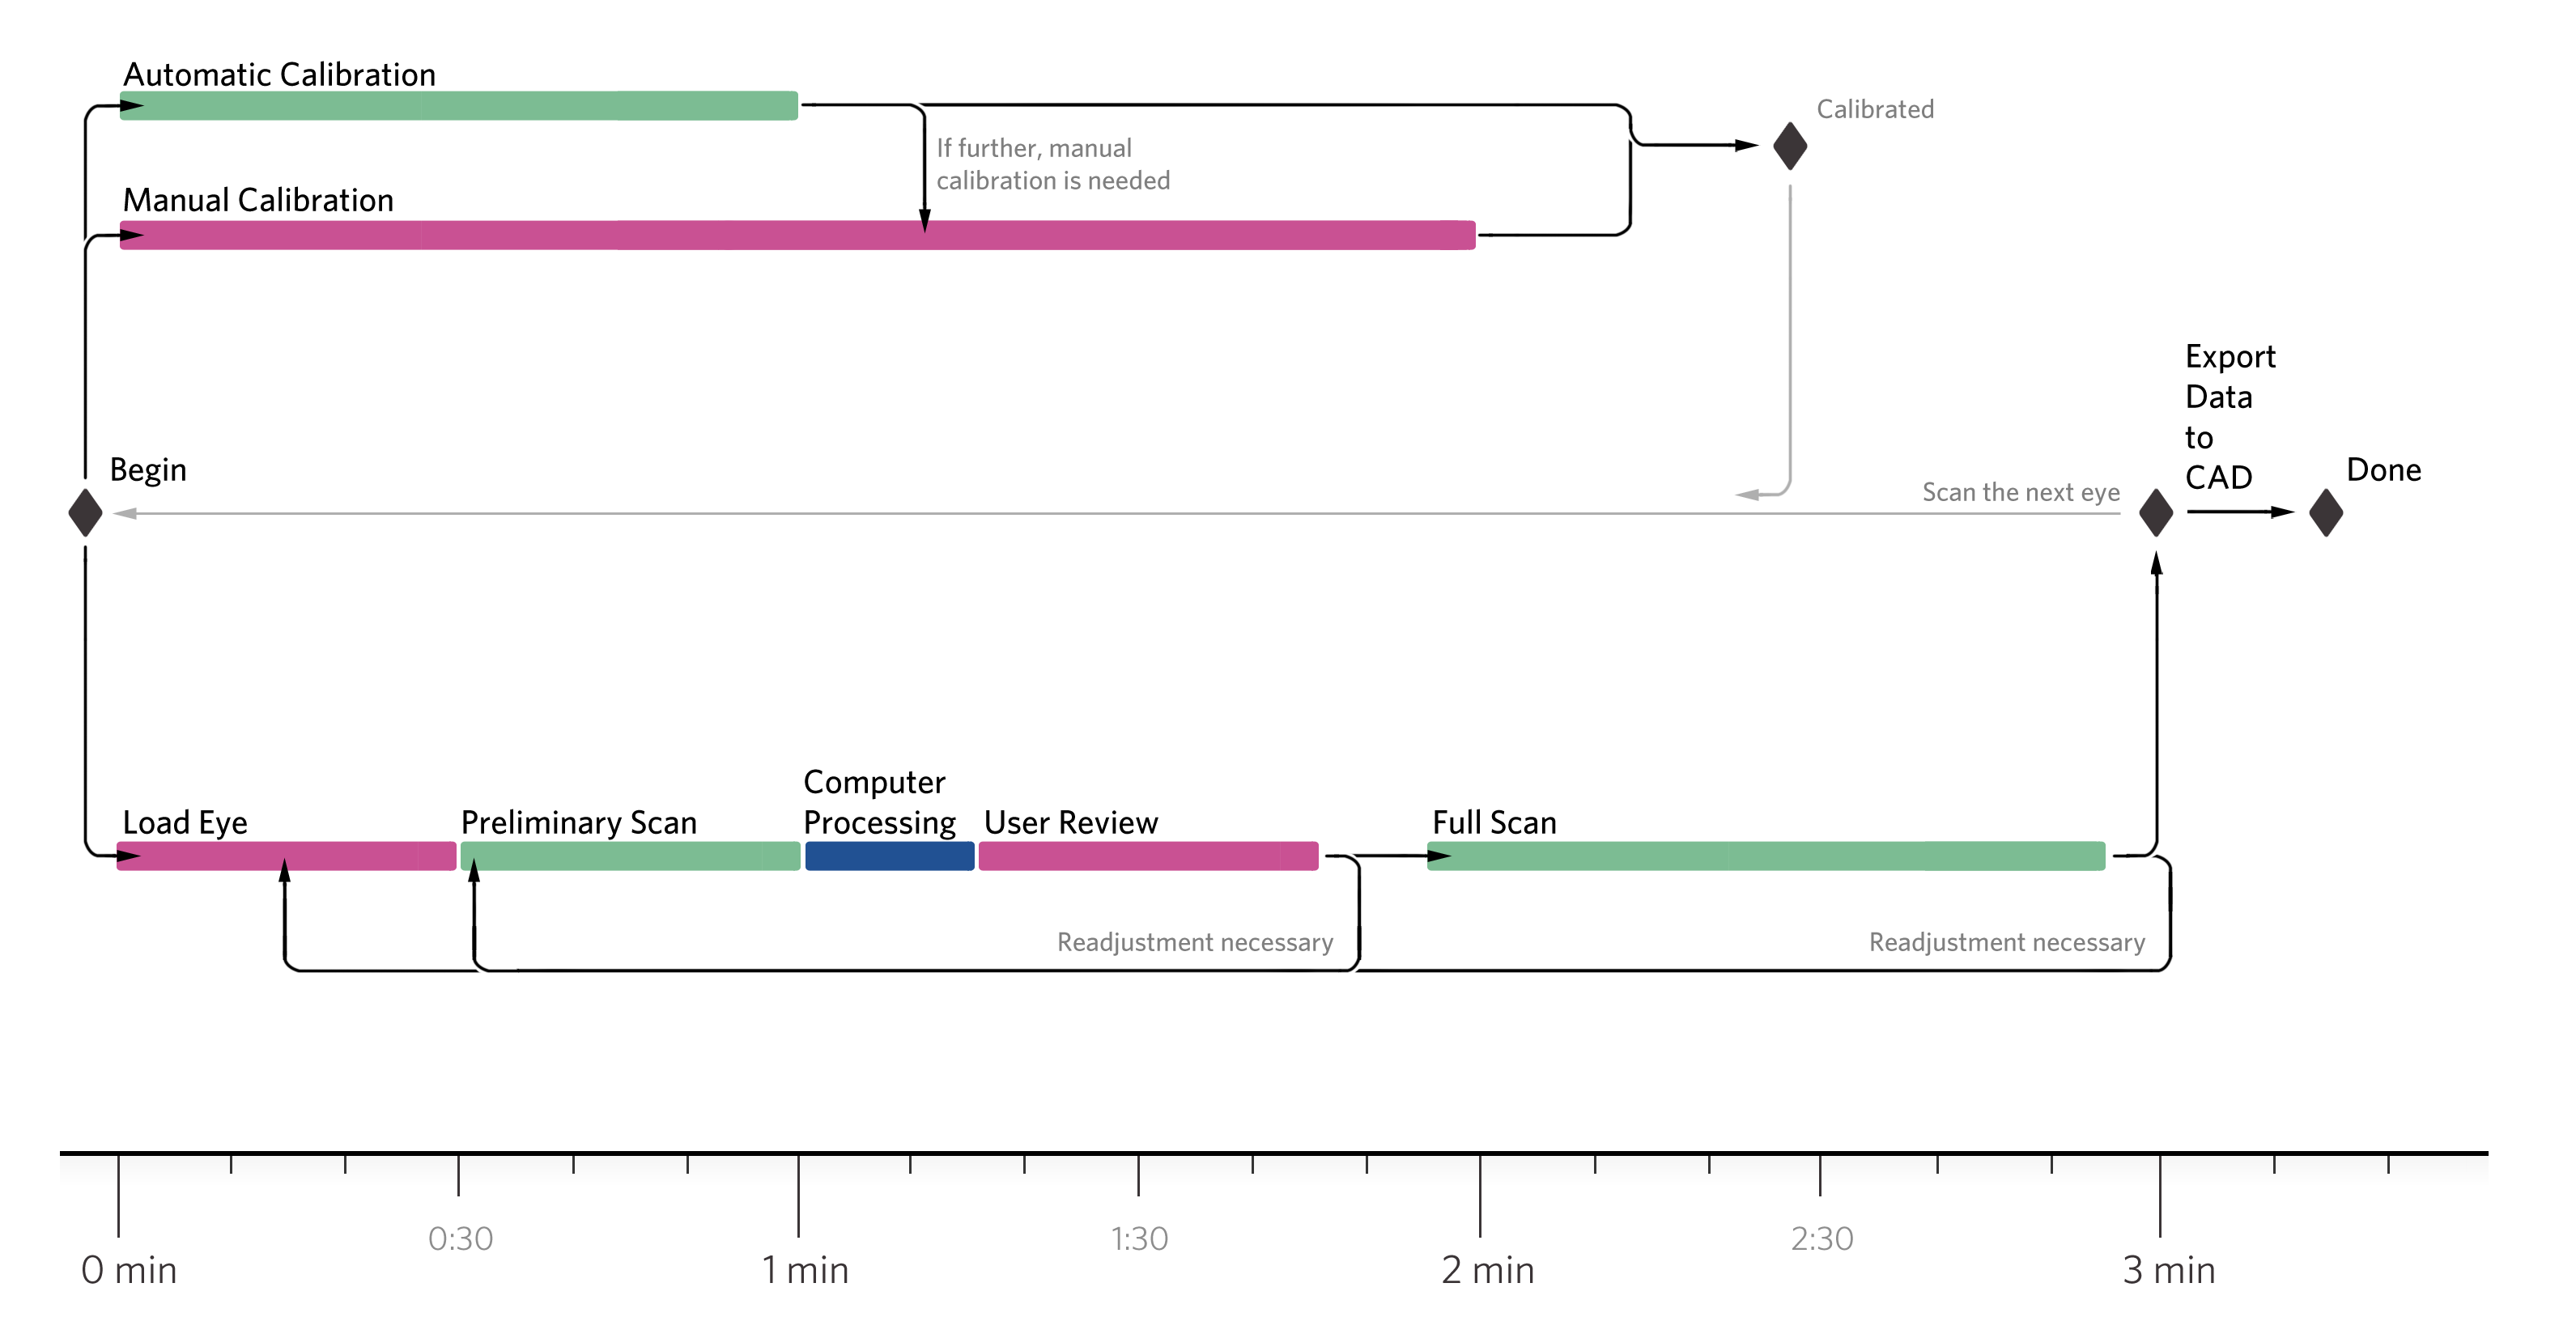
\includegraphics[width=\linewidth]{../img/usage_flow}
  \figcaption{\textbf{Possible usage flowchart for digitizer device.}  
  The device is controlled via the computer interface in order to perform a number of tasks required for repeatable, accurate measurement of an eye. Each task is located at and extended over the suggested period of time required to perform the task. Colors of the task boxes encode the required user interaction. Red tasks require direct user interaction with the physical harness, green tasks only require interaction with the computer, and blue tasks are computational tasks where the user must wait.}
  \label{fig:usage}
\end{figure}



\newpage
\bibliographystyle{unsrt}
\bibliography{../tex/bibl}

\end{document}
